\documentclass{article}
\usepackage[utf8]{inputenc}
\usepackage{geometry}
\usepackage{datetime2}
\usepackage{xparse}
\usepackage{amsmath}
\usepackage{booktabs}
\usepackage{array}
\usepackage{hyperref}


 \geometry{
 a4paper,
 total={170mm,257mm},
 left=20mm,
 top=20mm,
 }

 
 \usepackage{graphicx}
 \usepackage{titling}

 \title{"Tugas 2 Kecerdasan Buatan : Coding Fuzzy"}
% \author{Muhammad Qomaruz Zaman}
\date{11 March 2026}
 
 \usepackage{fancyhdr}
\fancypagestyle{plain}{%  the preset of fancyhdr 
    \fancyhf{} % clear all header and footer fields
    \fancyfoot[R]{}
    \fancyfoot[L]{}
    \fancyhead[L]{
\includegraphics[width=2cm]{ITS_pojok.pdf}}
    \fancyhead[R]{ \DTMnow}
}
\makeatletter
\def\@maketitle{%
  \newpage
  \null
  \vskip 1em%
  \begin{center}%
  \let \footnote \thanks
    {\LARGE \@title \par}%
    \vskip 1em%
    %{\large \@date}%
  \end{center}%
  \par
  \vskip 1em}
\makeatother

\usepackage{lipsum}  
% \usepackage{cmbright} % Change the font by zee

\begin{document}

\maketitle


\noindent\begin{tabular}{@{}ll}
    Author(s): & Irwnaysah Indra Prayoga\\
     Teacher: &  Muhammad Qomaruz Zaman, S.T., M.T., Ph.D.\\
     Class name: & Kecerdasan Buatan\\
     YouTube video link: & \url{https://youtu.be/XnGeqjbIusw?si=C58i2F8sJz37gfQx} \\
     GitHub link: & \url{https://github.com/dharmamangrwa/Tugas-Kecerdasan-Buatan-2.git}
\end{tabular}
\vspace{2cm}

\section*{Diketahui :}

\noindent\begin{tabular}{@{}ll}
    Diberikan persoalan sebagai berikut : (Figure 1)
\end{tabular}

\begin{figure}[tb]
    \begin{quote}
    \clearpage
    \centering{Persoalan :}
    \end{quote}
    \centering
    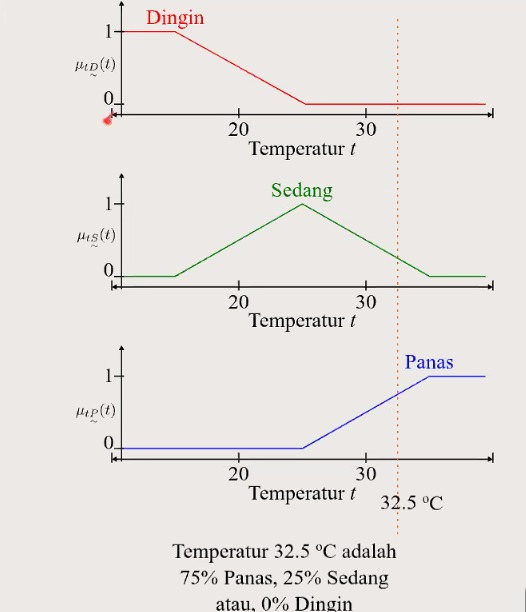
\includegraphics[width=0.5\linewidth]{Persoalan.jpeg}
    \caption{Soal 1}
    \label{fig:enter-label}
\end{figure}

\section*{Ditanya :}

\begin{enumerate}
\item Temperature 32.5 adalah 75 persen dengan kategori : Panas.
\item Temperature dengan persentase 25 persen dengan kategori : Sedang.
\item Temperature dengan persentase 0 persen dengan kategori : Dingin.
\item Buatkan Codingnya melalui google collab.
\end{enumerate}

\section*{Solusi :}

Didapatkan formula persamaan sebagai berikut : \begin{itemize}

\item def triangular(x, a, b, c):
\item    if x <= a or x >= c:
\item        return 0
\item    elif a < x <= b:
\item        return (x-a)/(b-a)
\item    elif b < x < c:
\item        return (c-x)/(c-b)

\item def trapezoid(x, a, b, c, d):
\item    if x <= a or x >= d:
\item        return 0
\item    elif a < x <= b:
\item        return (x-a)/(b-a)
\item    elif b < x <= c:
\item        return 1
\item    elif c < x < d:
\item        return (d-x)/(d-c)

Maka didapatkan hasil running pada google collab sebagai berikut = (Figure 2) 

\begin{figure}[tb]
    \begin{quote}
    \clearpage
    \centering{Dingin :}
    \end{quote}
    \centering
    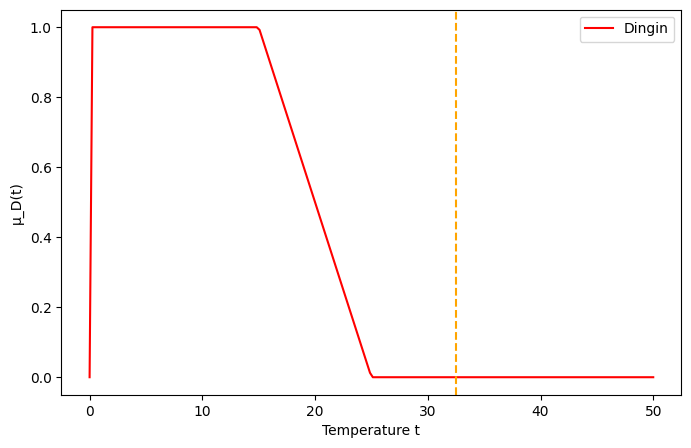
\includegraphics[width=0.5\linewidth]{download (1).png}
    \caption{Hasil Running Temperature Dingin}
    \label{fig:enter-label}
\end{figure}

\begin{figure}[tb]
    \begin{quote}
    \clearpage
    \centering{Sedang :}
    \end{quote}
    \centering
    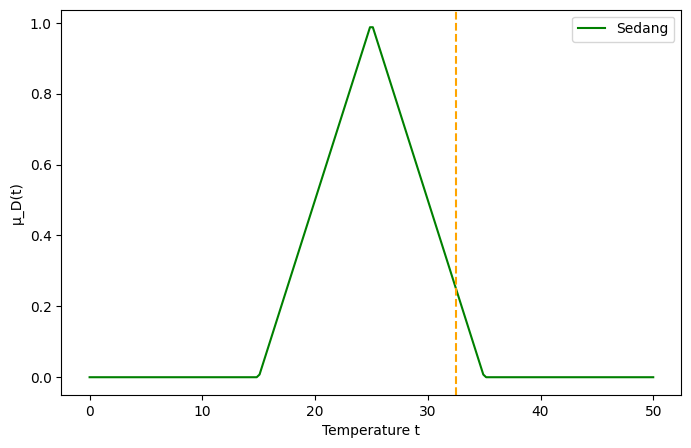
\includegraphics[width=0.5\linewidth]{download.png}
    \caption{Hasil Running Temperature Sedang}
    \label{fig:enter-label}
\end{figure}

\begin{figure}[tb]
    \begin{quote}
    \clearpage
    \centering{Panas :}
    \end{quote}
    \centering
    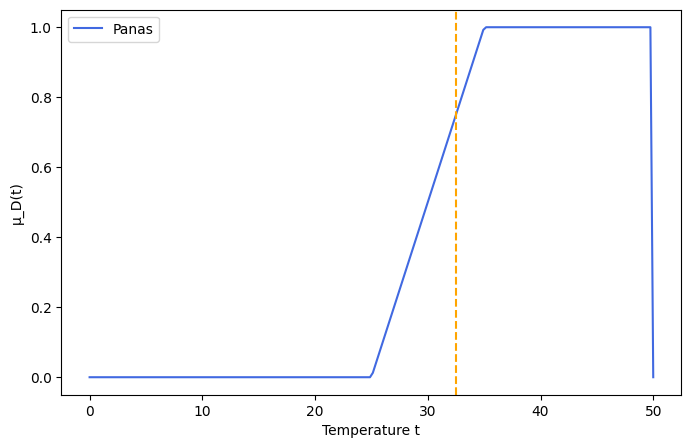
\includegraphics[width=0.5\linewidth]{download (2).png}
    \caption{Hasil Running Temperature Panas}
    \label{fig:enter-label}
\end{figure}


\end{document}
